\pagenumbering{gobble}
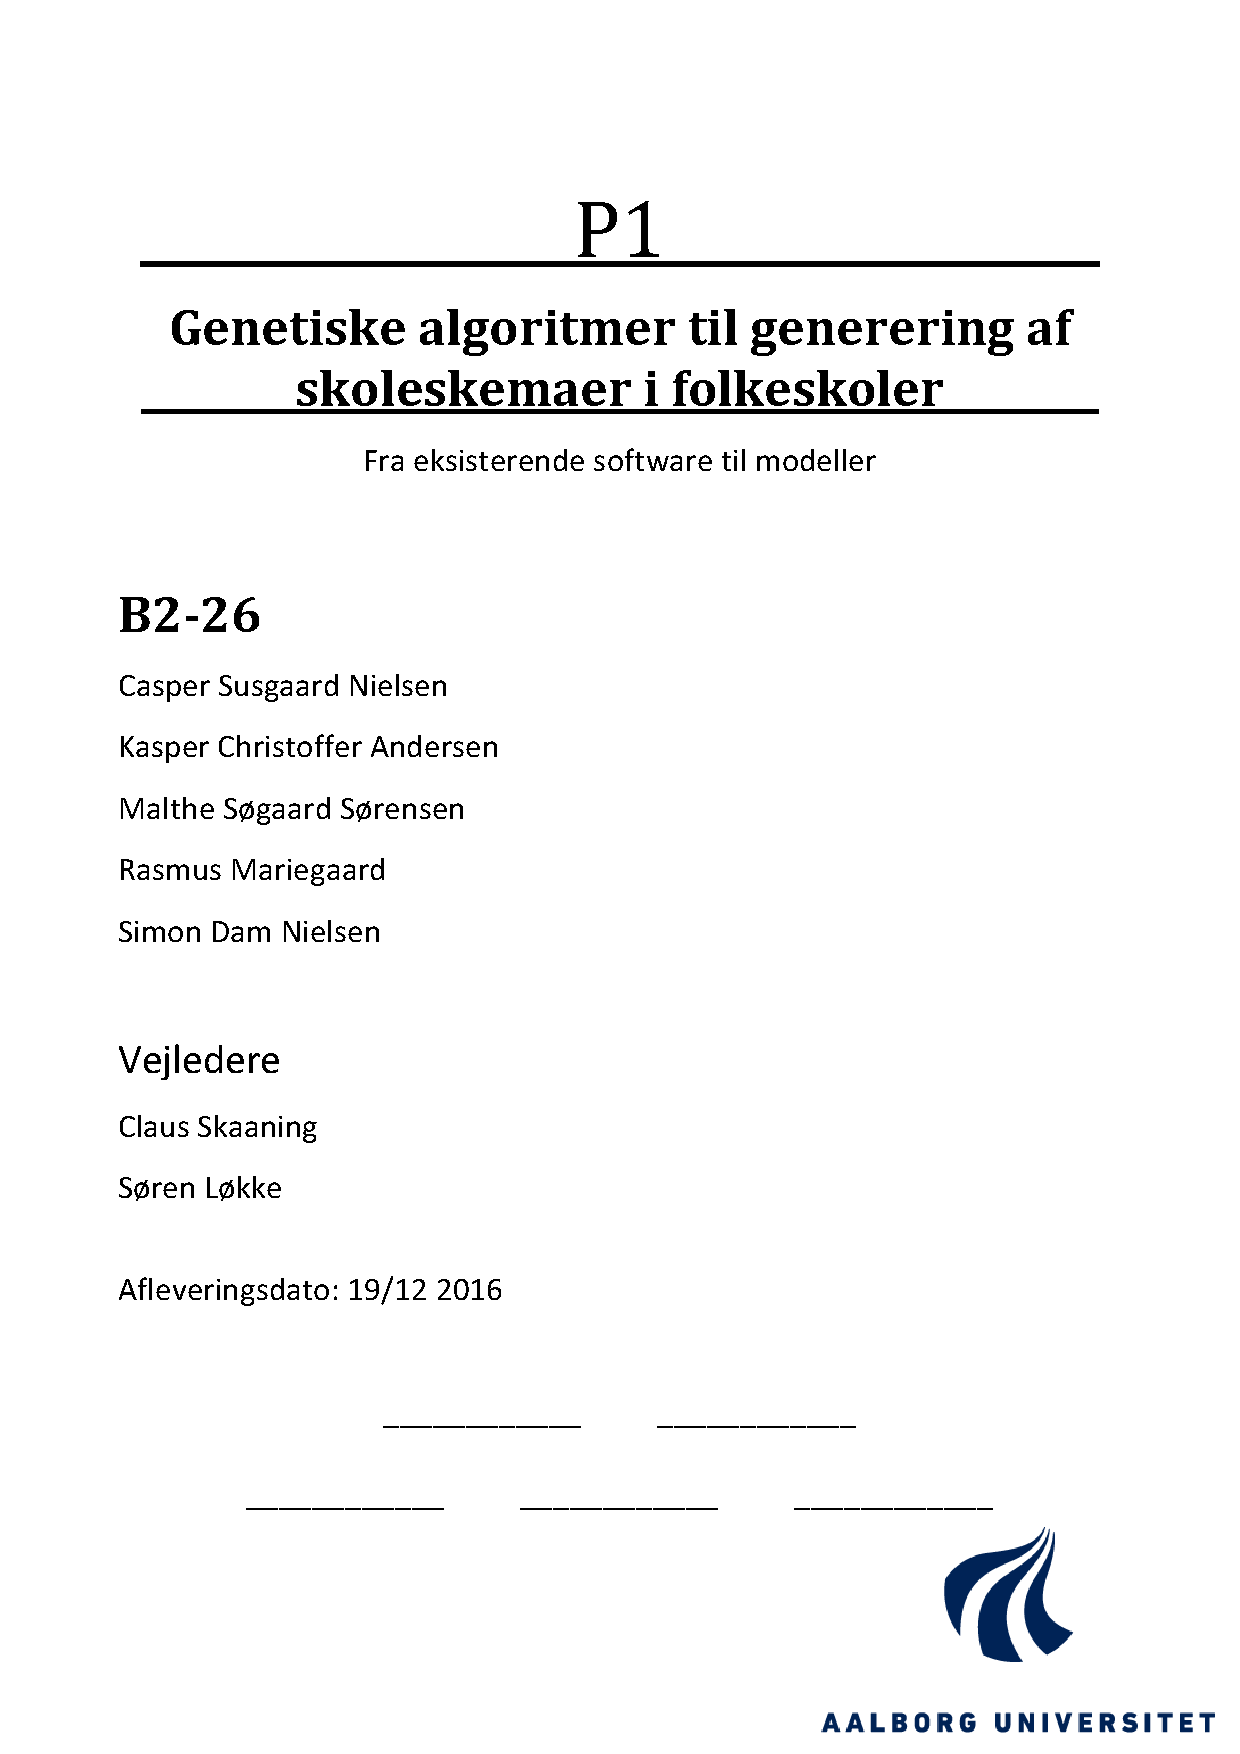
\includepdf[pages={1}]{partials/graphics/forside.pdf}
\clearpage
\pagenumbering{arabic}
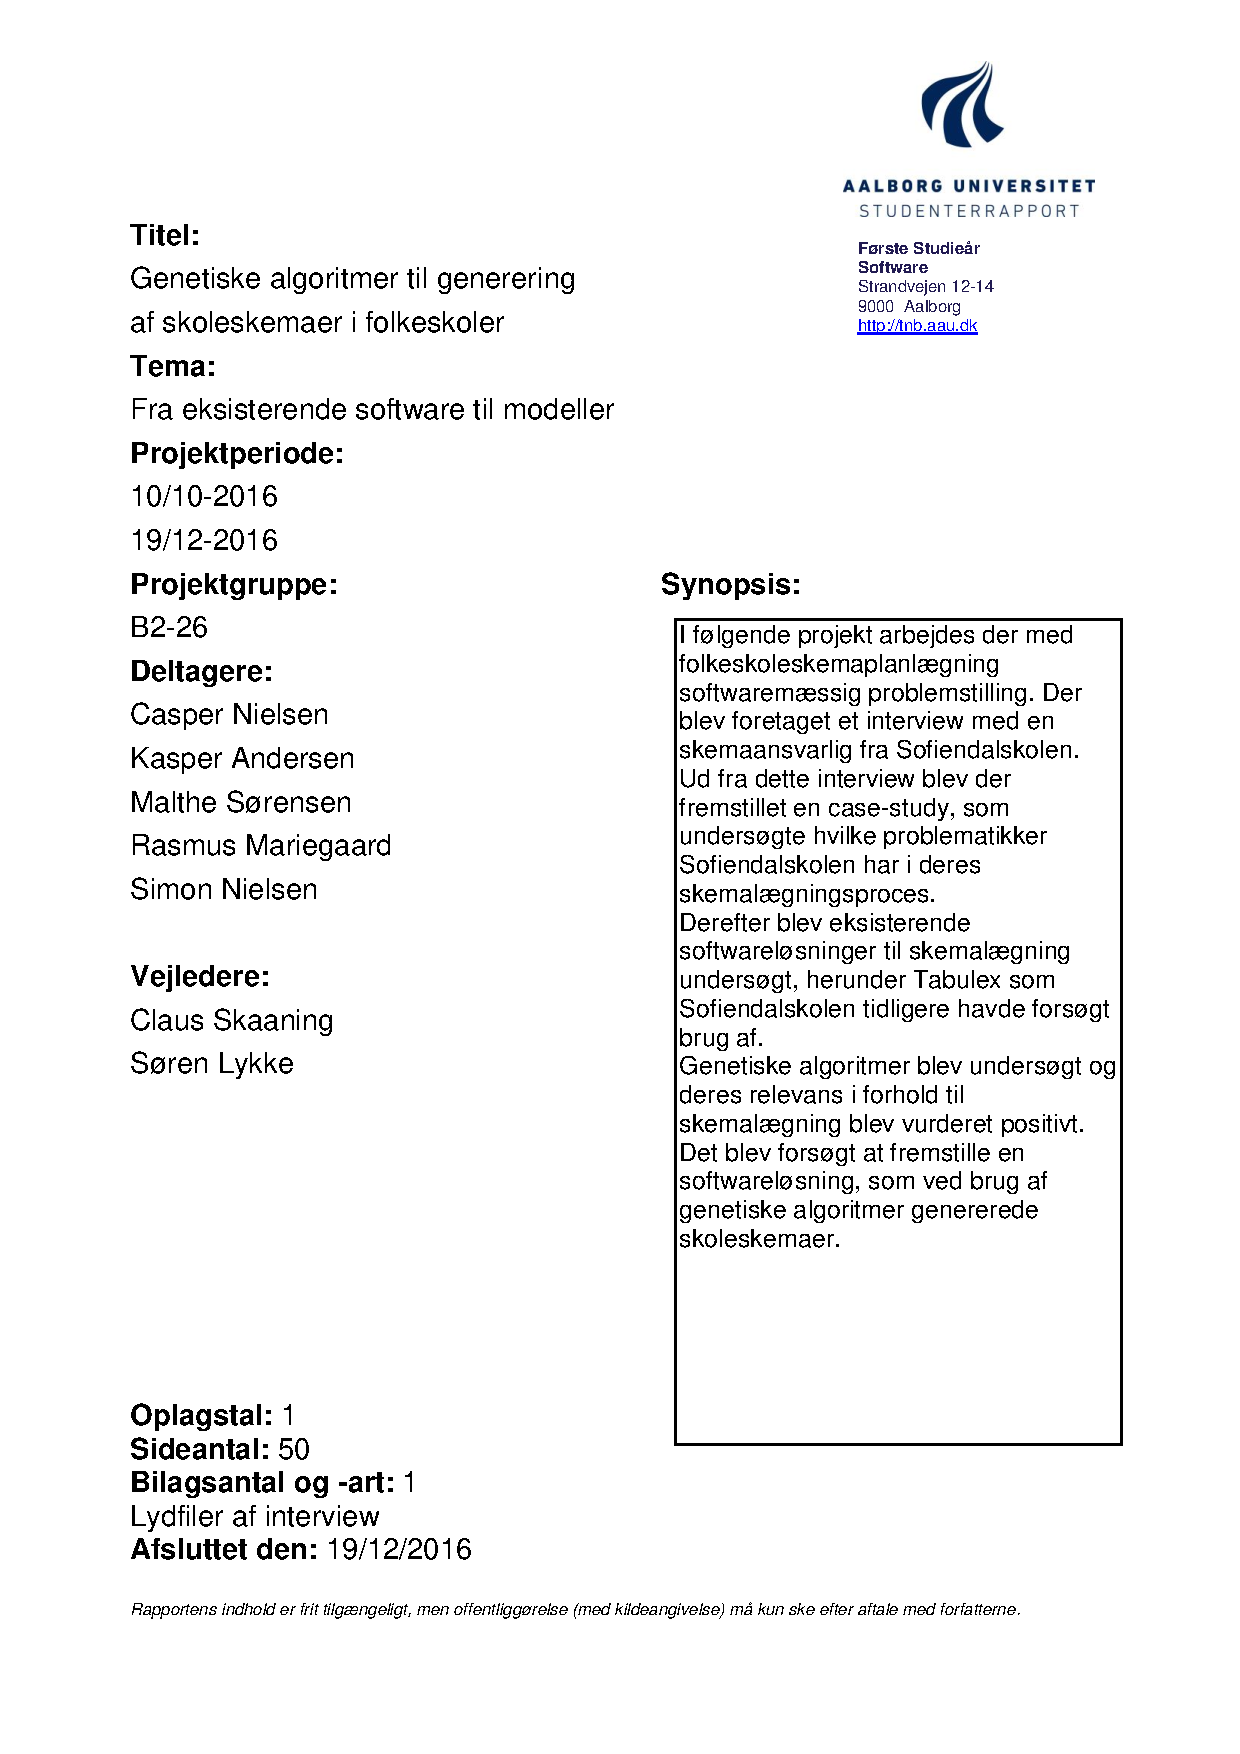
\includepdf[pages={1}]{partials/graphics/synopsis_Software.pdf}
\clearpage
\setcounter{page}{1}
\section{Forord}
Vi vil gerne takke Sofiendalskolen for at lade os interviewe Søren Kusk, og specielt tak til Søren Kusk for hans tid.

\section{Abstract}
The following project examines the use of genetic algorithms for use in the process of planning elementary school schedules. An interview with a schedule planner from Sofiendalskolen was conducted. From this interview a case-study was produced, which examined the problems which occurred in the scheduling process in Sofiendalskolen. Existing scheduling programs were examined afterwards, once of which were Tabulex, a program Sofiendalskolen previously had attempted to use. Genetic algorithms relevance was examined in context of the planning of school schedules. It was concluded to be adequate for generating school schedules. An attempt was made to produce a software solution which used genetic algorithms to generate school schedules. The software solution was concluded to produce an adequate schedule, but with an ineffective genetic algorithm. 
\newpage
\tableofcontents
\newpage
